\subsection{Implementación elegida}

Elegimos utilizar la meta-heurística GRASP con el algoritmo goloso aleatorizado
en la elección de aristas, eligiendo al azar una de las 10 más pesadas en cada
iteración.

Luego aplicándole el algoritmo de búsqueda local que denominamos \textit{mover}, que
define como vecindades a todas las particiones que difieren de la actual por
tener un único vértice en un conjunto distinto.

Finalmente veremos los dos criterios de terminación:
\begin{itemize}
  \item repitiendo hasta que la mejor solución se encuentre 34 veces.
  \item repitiendo exactamente 47 veces y quedándonos con la mejor hasta el momento.
\end{itemize}

\subsection{Otras implementaciones para contrastar}

Vamos a contrastar los resultados contra las siguientes implementaciones:

\begin{itemize}
  \item Exacto (mientras el tiempo de ejecución sea menor a 5 minutos).
  \item Goloso sin aleatorizar.
  \item GRASP, pero aleatorizando tanto aristas como conjuntos.
  \item GRASP, pero utilizando el algoritmo de búsqueda local
  \textit{intercambiar}.
\end{itemize}

\subsection{Experimentación}

Experimentamos con distintos tipos de grafos, variando la cantidad de vértices,
variando la cantidad de aristas según el grafo, con dos cantidades de conjuntos
distintas y, para cada combinación de valores, generar 15 grafos distintos.

Analicemos primero los tiempos:

Árbol, k=3

\begin{figure}[H]
  \begin{center}
    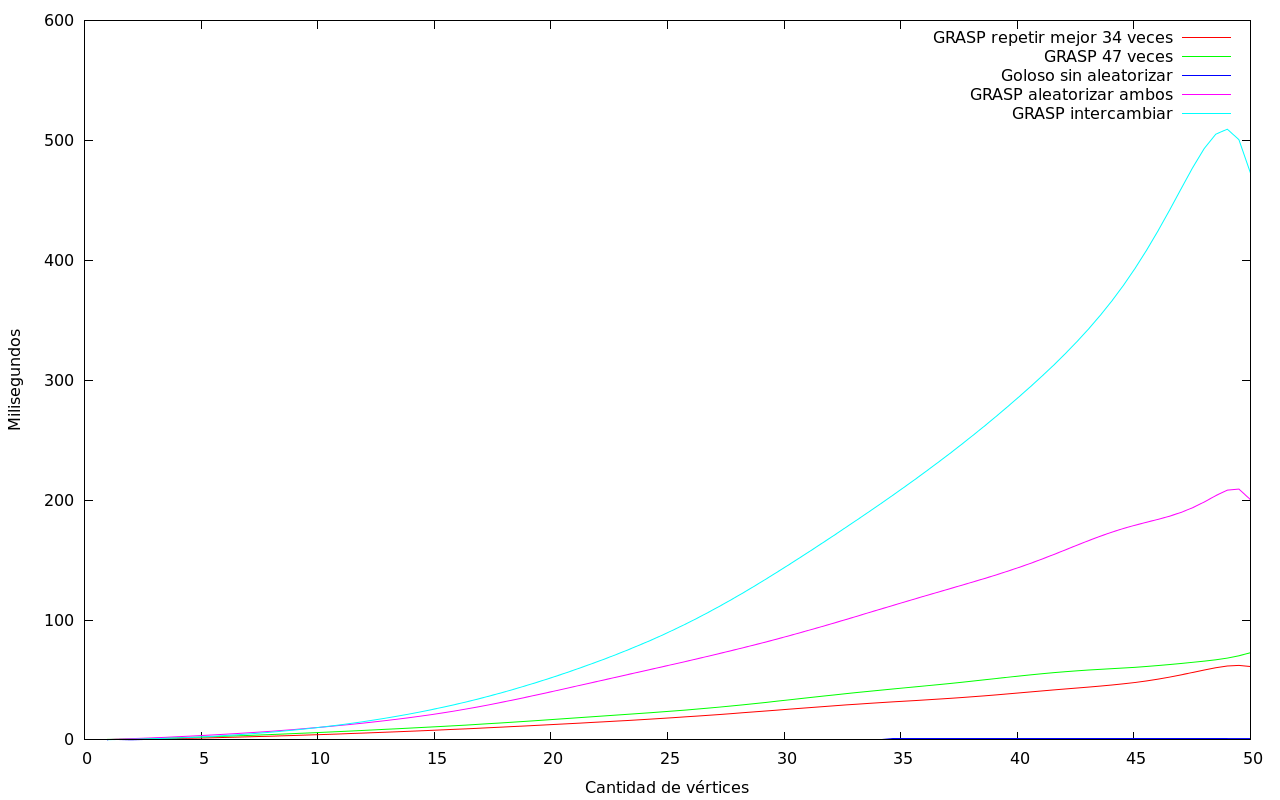
\includegraphics[scale=0.35]{imagenes/ej6-arbol-k3-tiempo.png}
  \end{center}
\end{figure}

Árbol, k=7

\begin{figure}[H]
  \begin{center}
    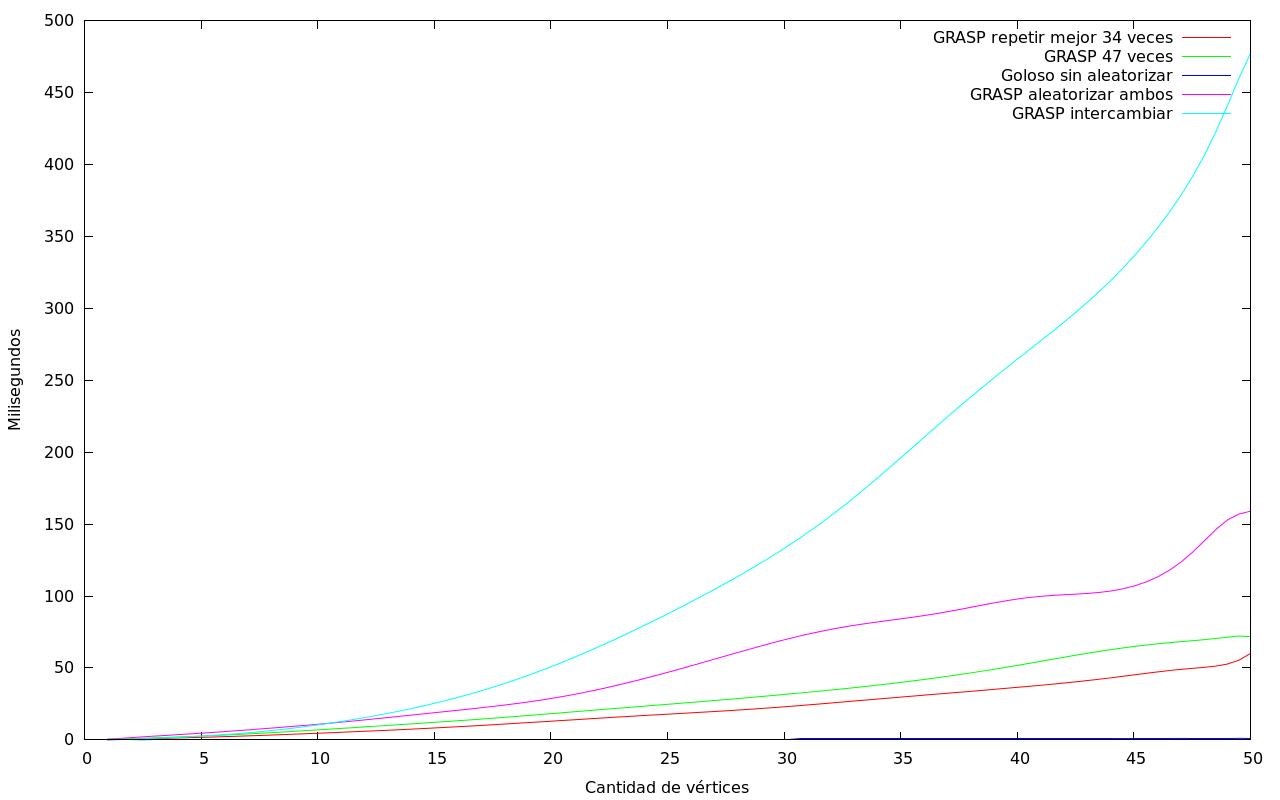
\includegraphics[scale=0.35]{imagenes/ej6-arbol-k7-tiempo.png}
  \end{center}
\end{figure}

Completo, k=3

\begin{figure}[H]
  \begin{center}
    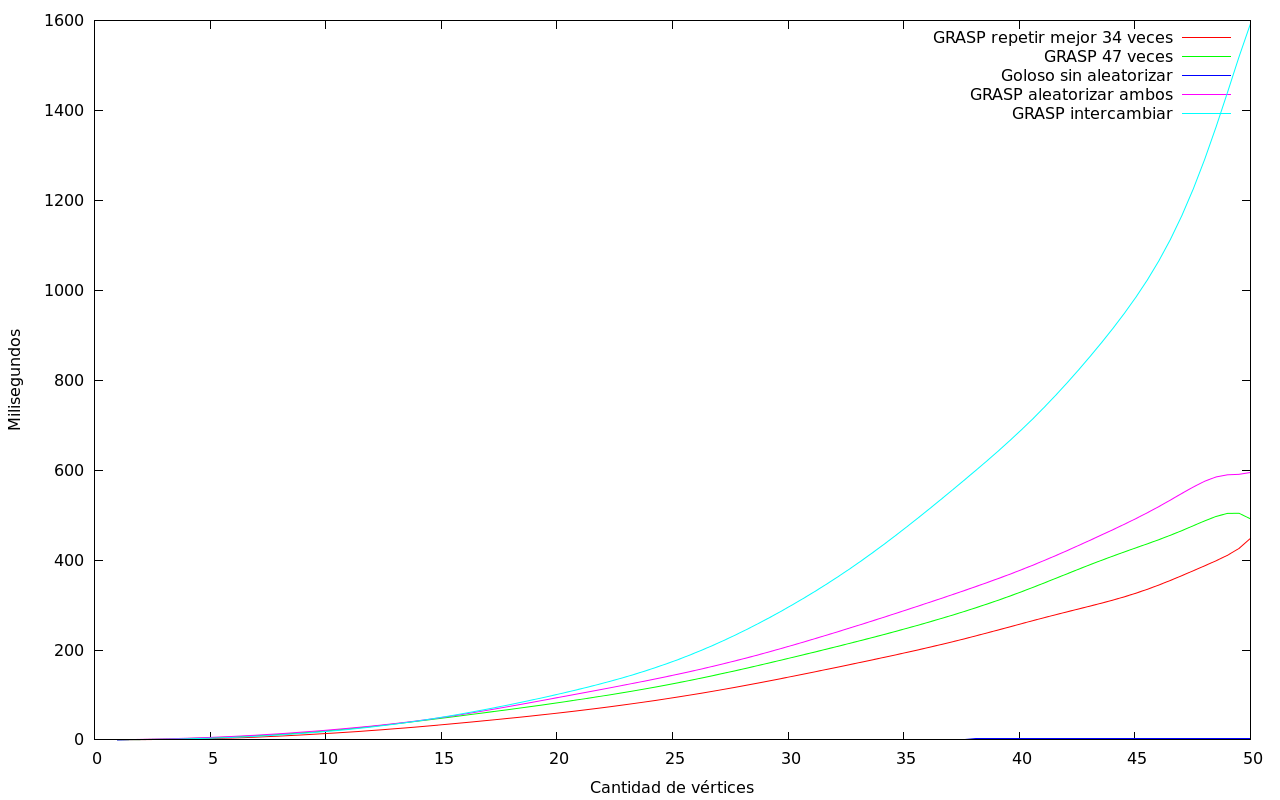
\includegraphics[scale=0.35]{imagenes/ej6-completo-k3-tiempo.png}
  \end{center}
\end{figure}

Completo, k=7

\begin{figure}[H]
  \begin{center}
    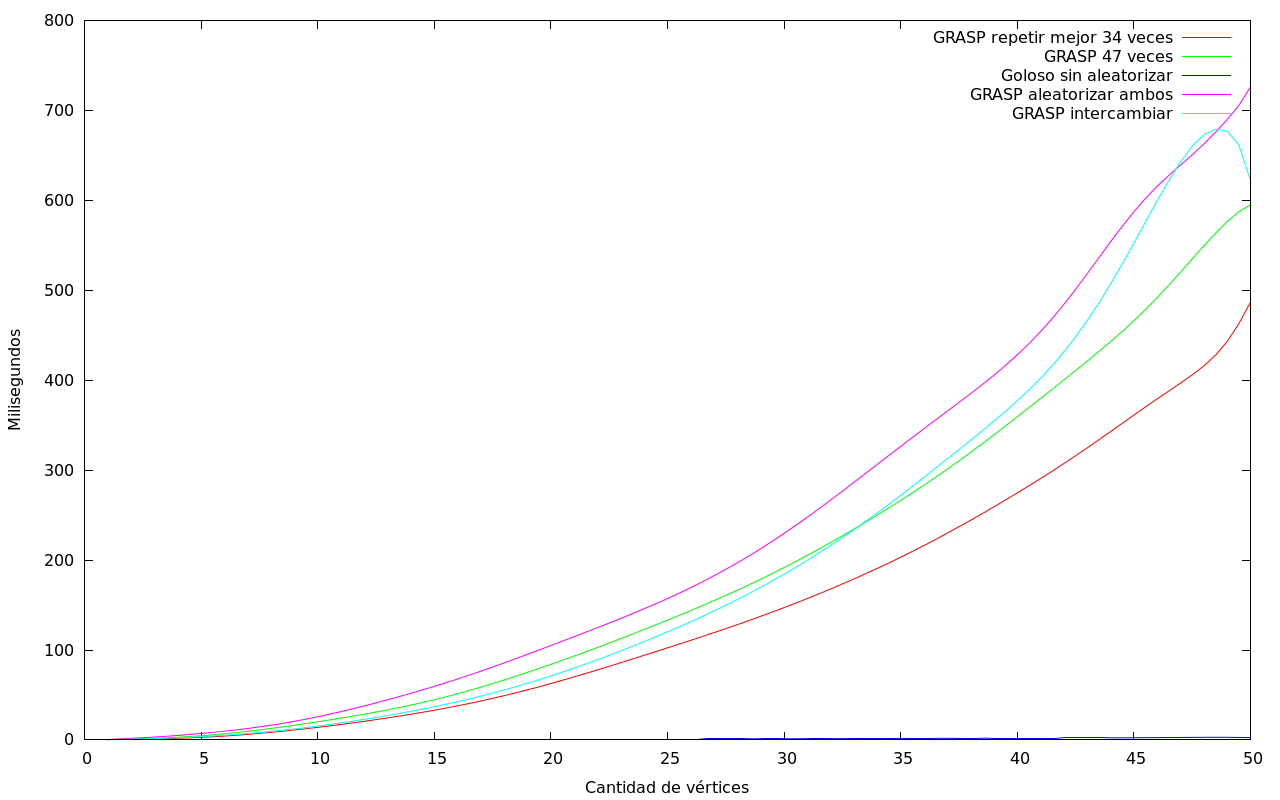
\includegraphics[scale=0.35]{imagenes/ej6-completo-k7-tiempo.png}
  \end{center}
\end{figure}

Denso, aristas con pesos iguales, k=3

\begin{figure}[H]
  \begin{center}
    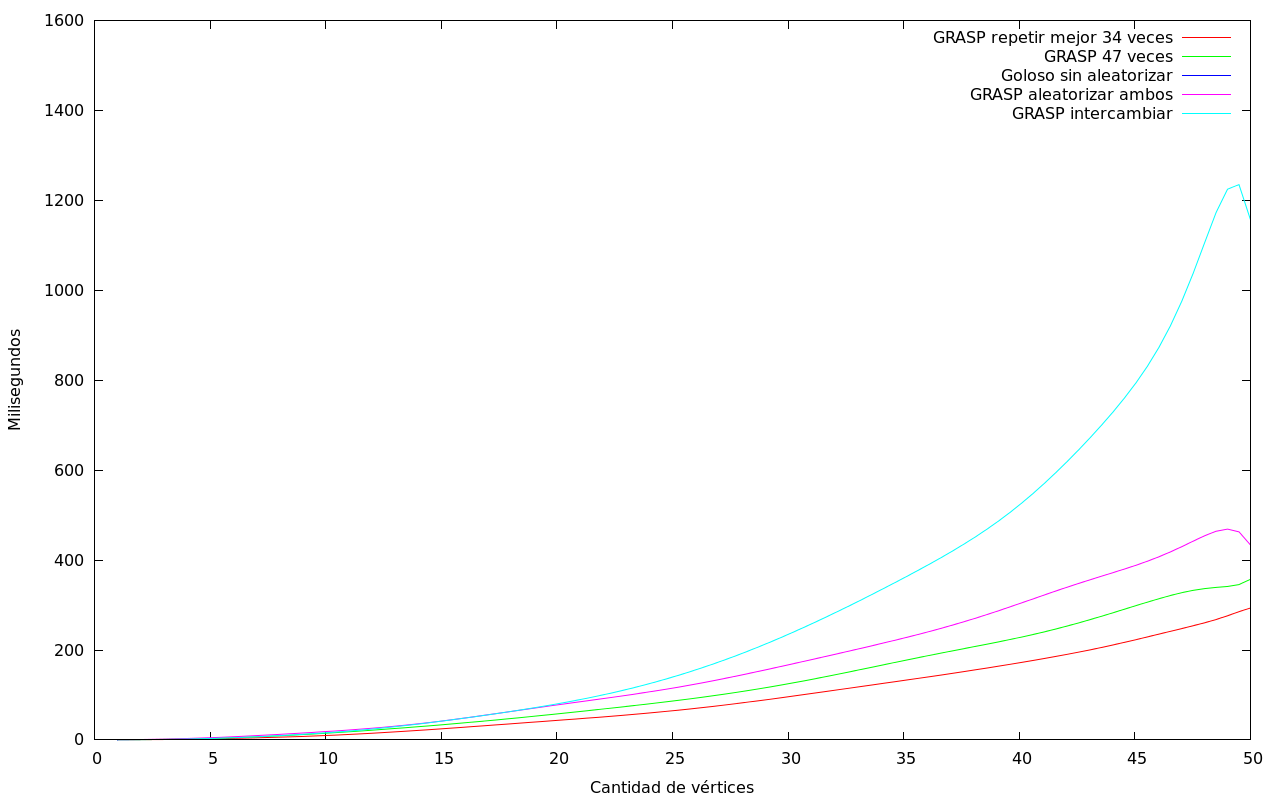
\includegraphics[scale=0.35]{imagenes/ej6-denso-pesos-iguales-k3-tiempo.png}
  \end{center}
\end{figure}

Denso, aristas con pesos iguales, k=7

\begin{figure}[H]
  \begin{center}
    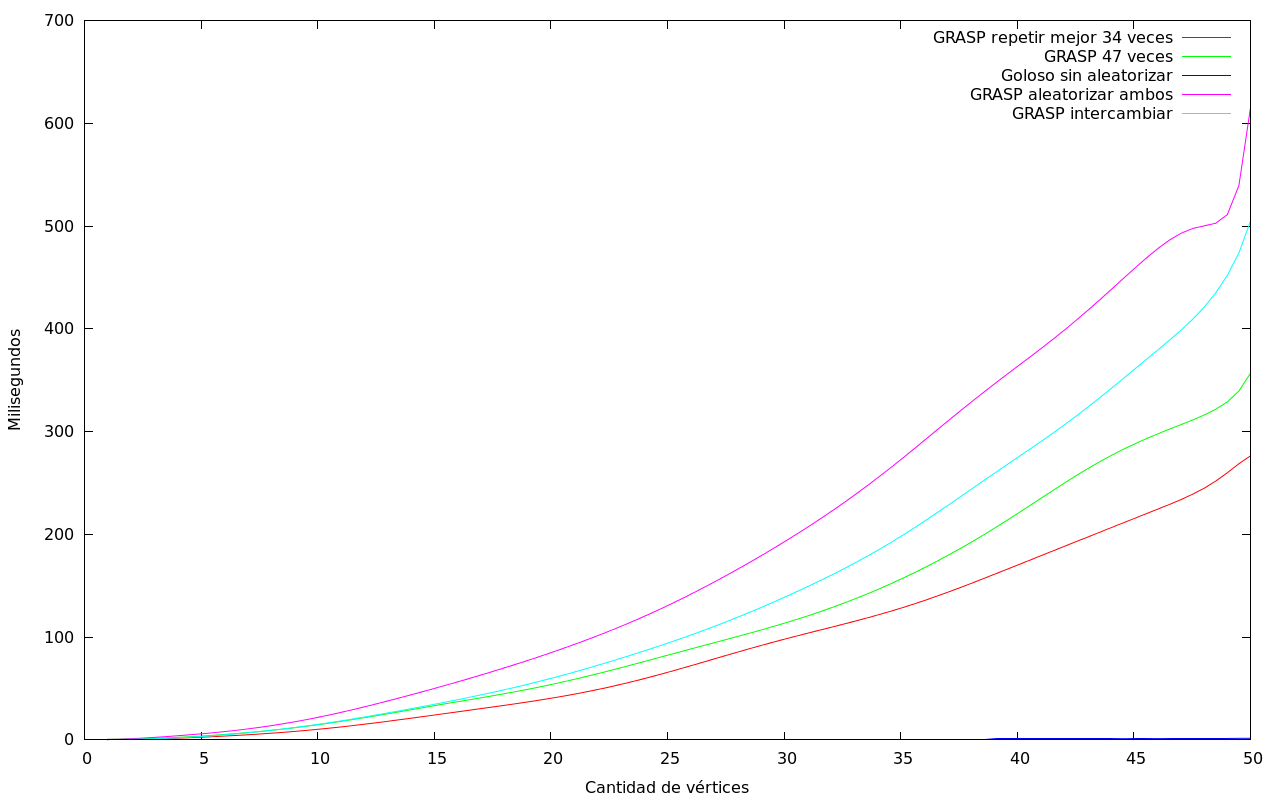
\includegraphics[scale=0.35]{imagenes/ej6-denso-pesos-iguales-k7-tiempo.png}
  \end{center}
\end{figure}

Denso, aristas con pesos distintos, k=3

\begin{figure}[H]
  \begin{center}
    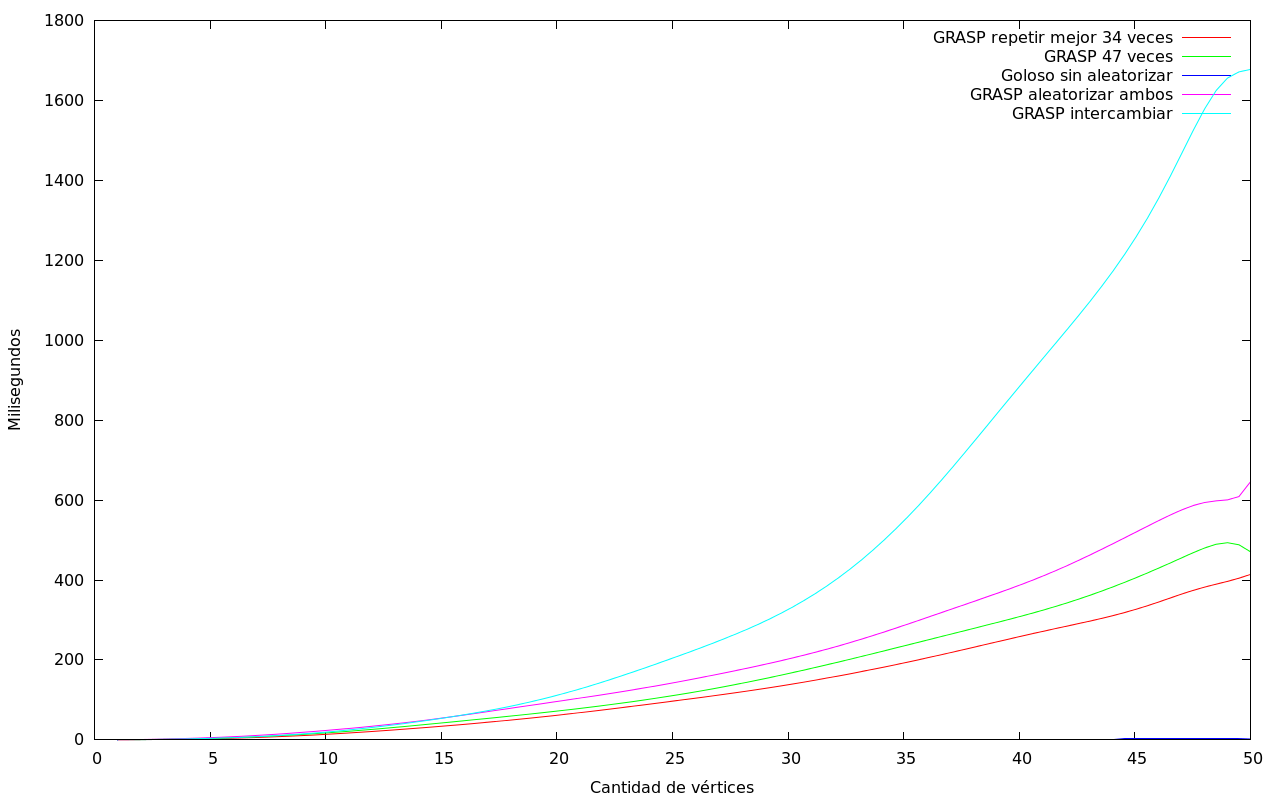
\includegraphics[scale=0.35]{imagenes/ej6-denso-pesos-distintos-k3-tiempo.png}
  \end{center}
\end{figure}

Denso, aristas con pesos distintos, k=7

\begin{figure}[H]
  \begin{center}
    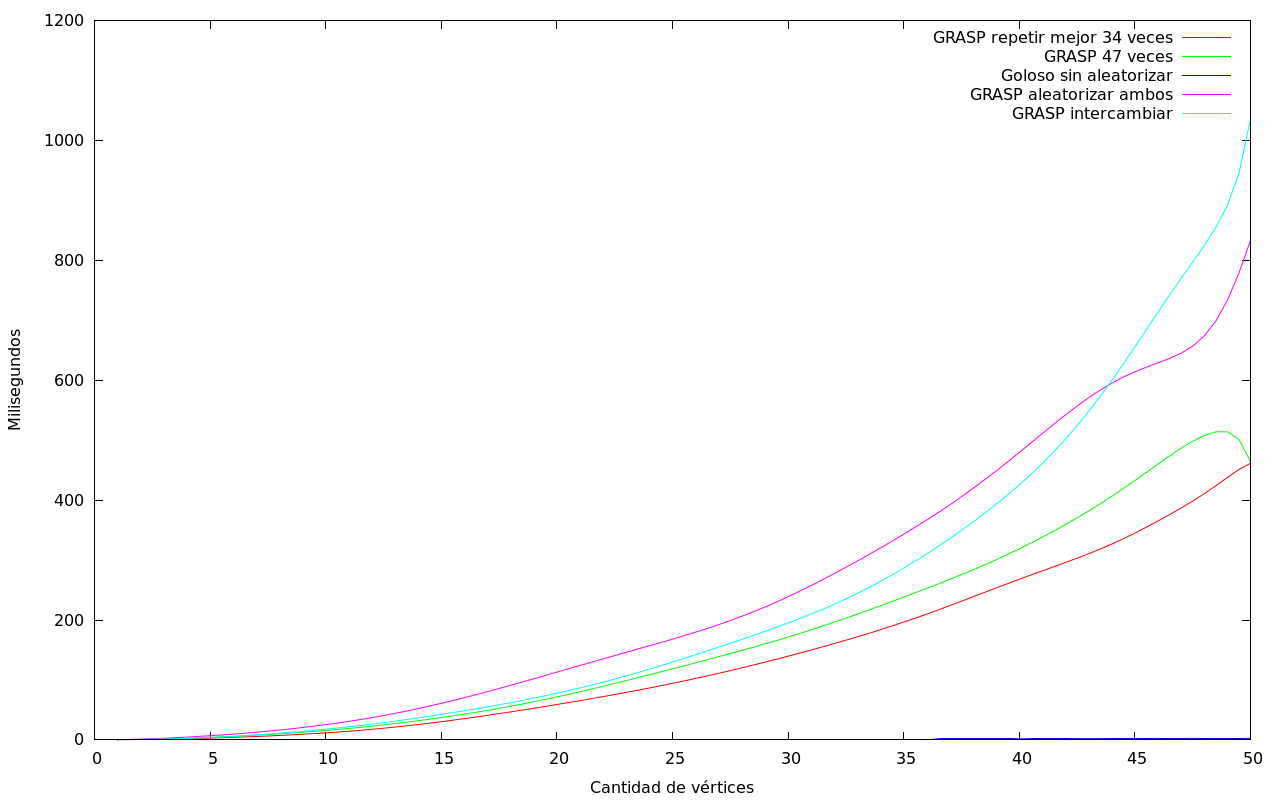
\includegraphics[scale=0.35]{imagenes/ej6-denso-pesos-distintos-k7-tiempo.png}
  \end{center}
\end{figure}

Aunque es difícil de graficar bien, el exacto crece mucho más rápido que todos
los otros algoritmos.  Lo ejecutamos hasta $n = 18$, pero para que se puedan
ver el resto de las líneas, a veces, lo cortamos incluso antes, como puede
verse en el gráfico del grafo completo con $k = 7$.

Eso puede hacer aparentar, en algunos casos (como en el gráfico de árbol con
$k = 3$), que el exacto crece más lento, pero en realidad es que si agregáramos
uno o más puntos, crecería tanto que el resto de las líneas parecerían rectas
sobre el 0.

Lo primero que se puede notar es que el goloso sin aleatorizar es el más
rápido, algo completamente esperable, ya que se ejecuta solamente una vez
contra la ejecución de la heurística local y repetida decenas de veces en el
GRASP.

Luego, también se observa que el peor de los GRASP es que utiliza la heurística
local de \textit{intercambiar}, seguido del algoritmo GRASP que aleatoriza
tanto aristas como conjuntos.

Los dos algoritmos elegidos son los que menor tiempo tardan (exceptuando el
goloso puro), con una pequeña ventaja el que realiza menos repeticiones.

Sin embargo, todavía falta contrastar la calidad de estos:

Árbol, k=3

\begin{figure}[H]
  \begin{center}
    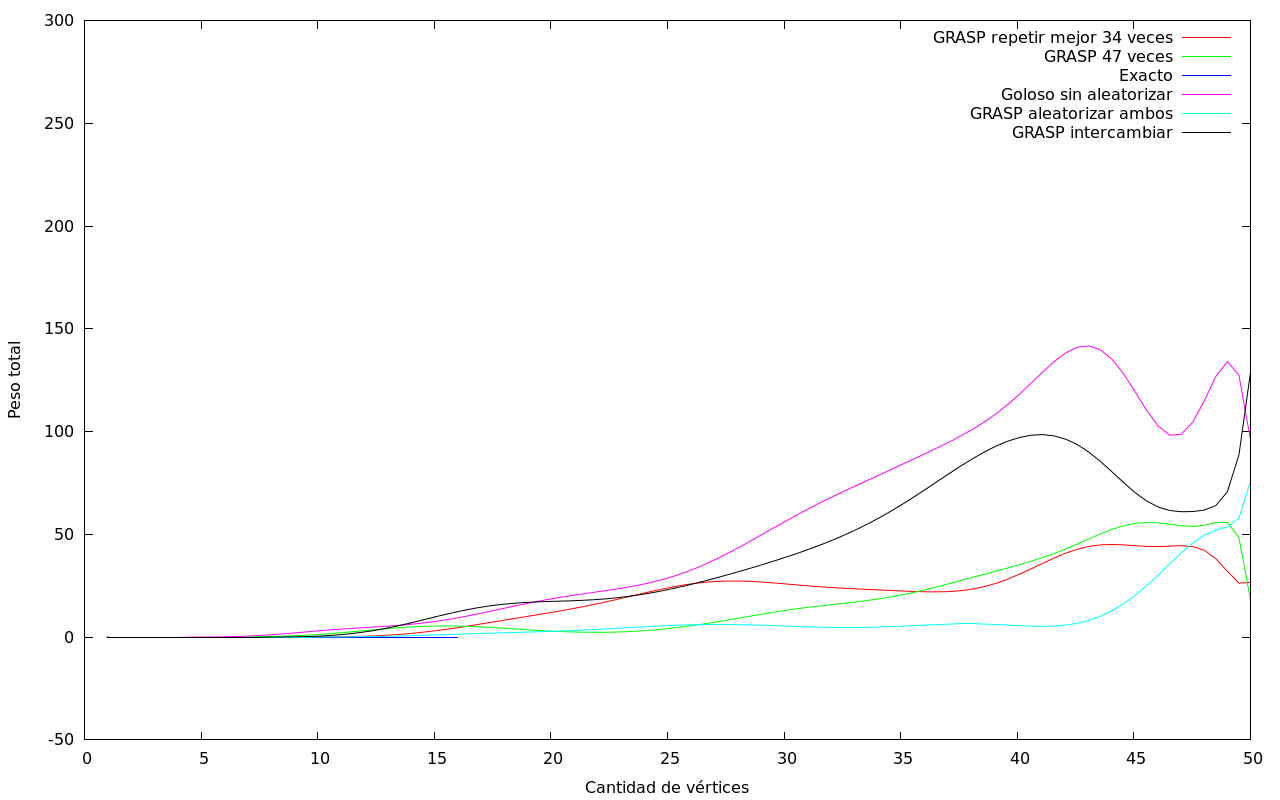
\includegraphics[scale=0.35]{imagenes/ej6-arbol-k3-peso.png}
  \end{center}
\end{figure}

Completo, k=3

\begin{figure}[H]
  \begin{center}
    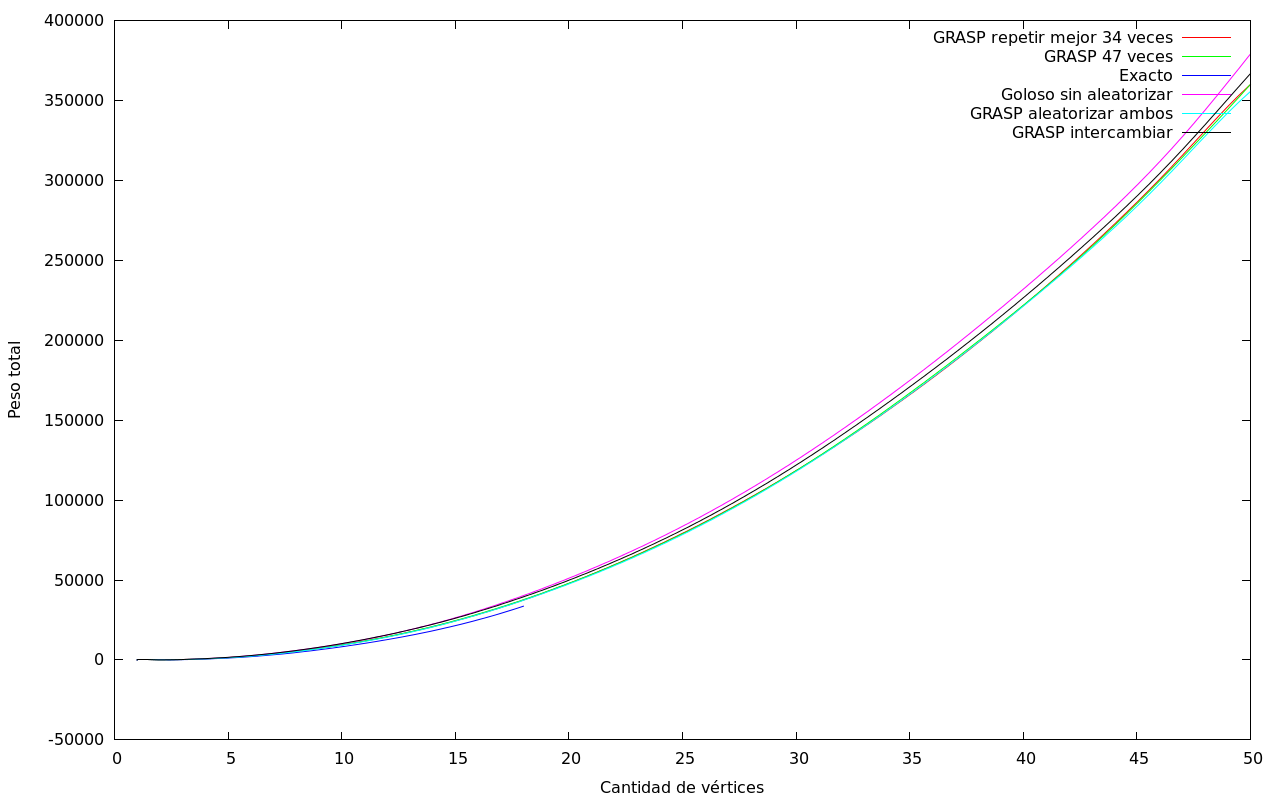
\includegraphics[scale=0.35]{imagenes/ej6-completo-k3-peso.png}
  \end{center}
\end{figure}

Completo, k=7

\begin{figure}[H]
  \begin{center}
    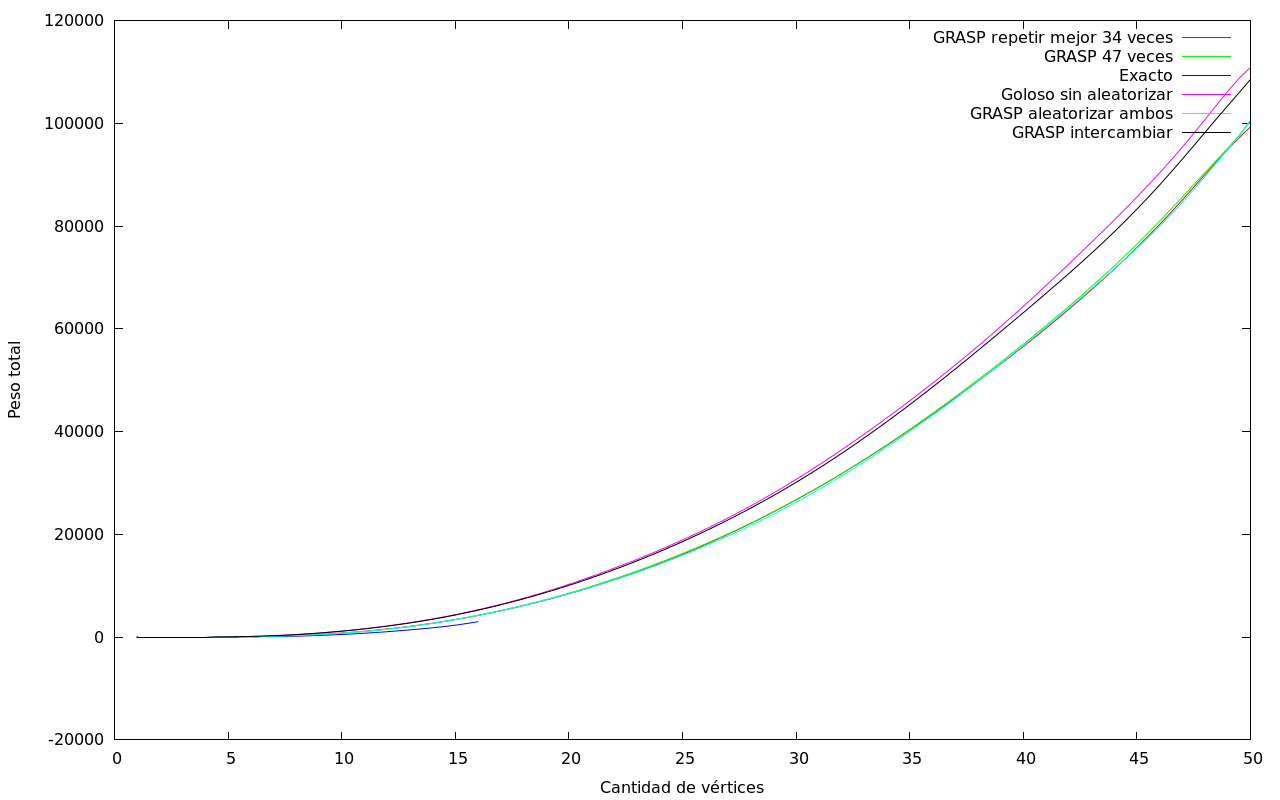
\includegraphics[scale=0.35]{imagenes/ej6-completo-k7-peso.png}
  \end{center}
\end{figure}

Denso, aristas con pesos iguales, k=3

\begin{figure}[H]
  \begin{center}
    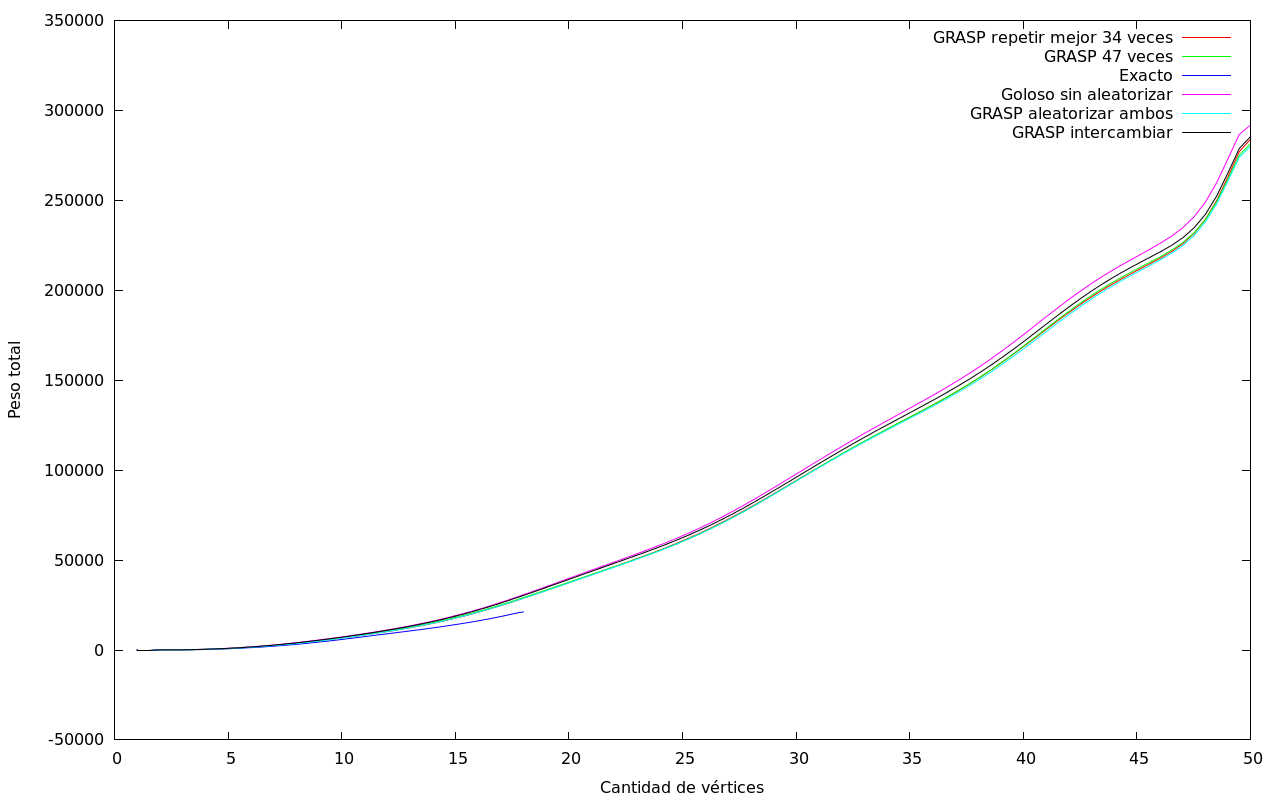
\includegraphics[scale=0.35]{imagenes/ej6-denso-pesos-iguales-k3-peso.png}
  \end{center}
\end{figure}

Denso, aristas con pesos iguales, k=7

\begin{figure}[H]
  \begin{center}
    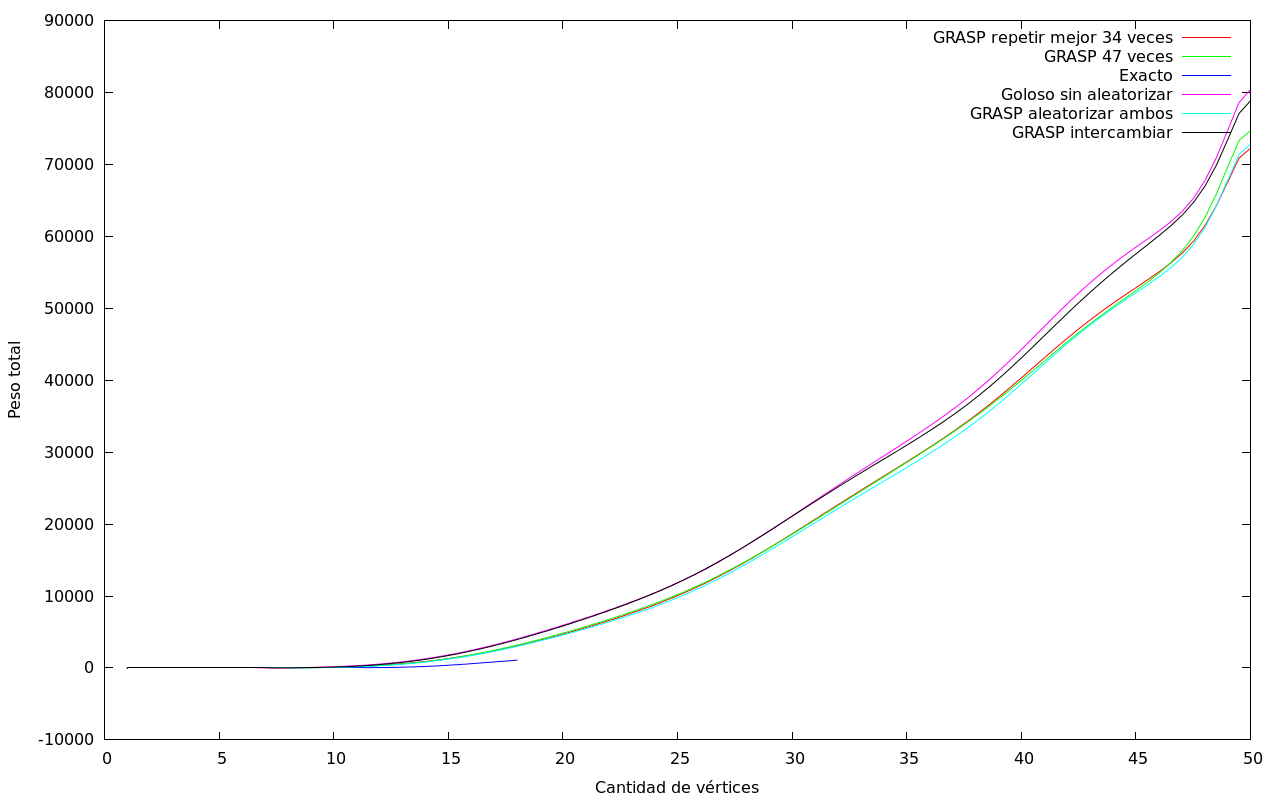
\includegraphics[scale=0.35]{imagenes/ej6-denso-pesos-iguales-k7-peso.png}
  \end{center}
\end{figure}

Denso, aristas con pesos distintos, k=3

\begin{figure}[H]
  \begin{center}
    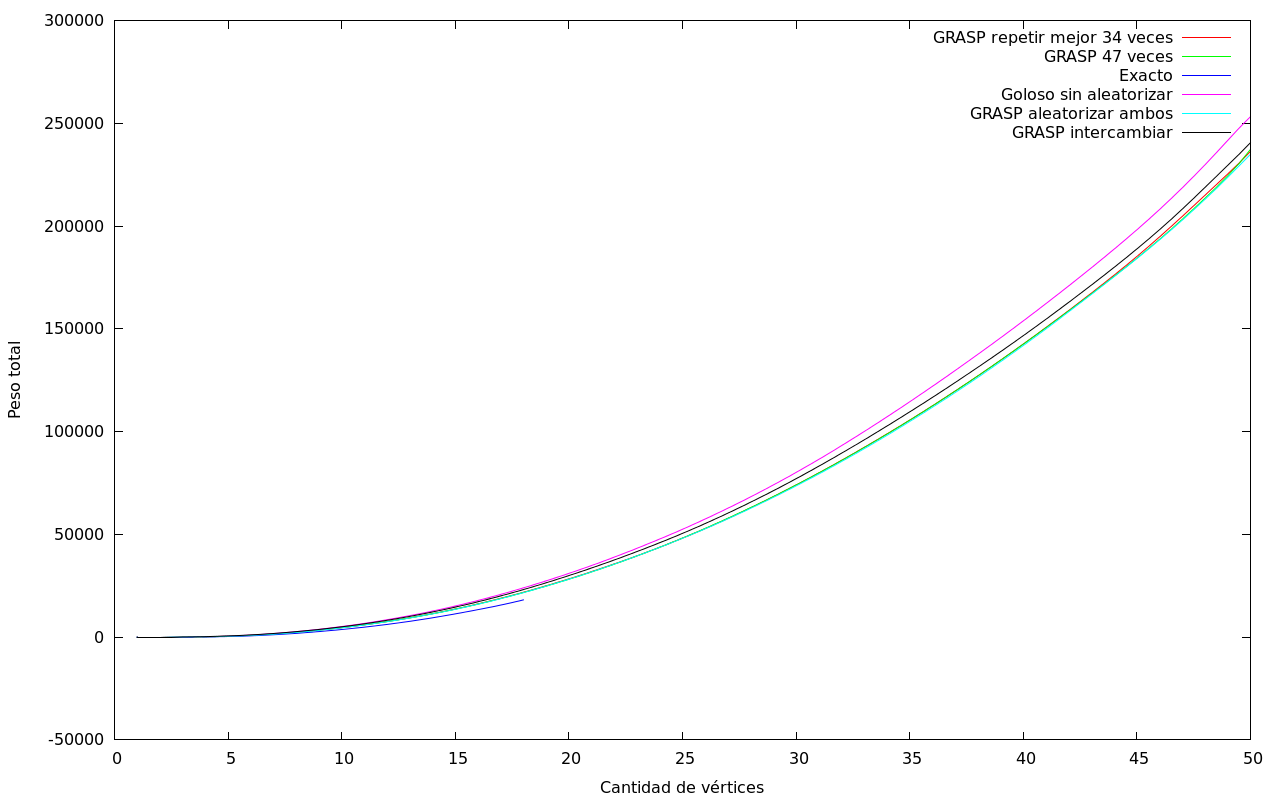
\includegraphics[scale=0.35]{imagenes/ej6-denso-pesos-distintos-k3-peso.png}
  \end{center}
\end{figure}

Denso, aristas con pesos distintos, k=7

\begin{figure}[H]
  \begin{center}
    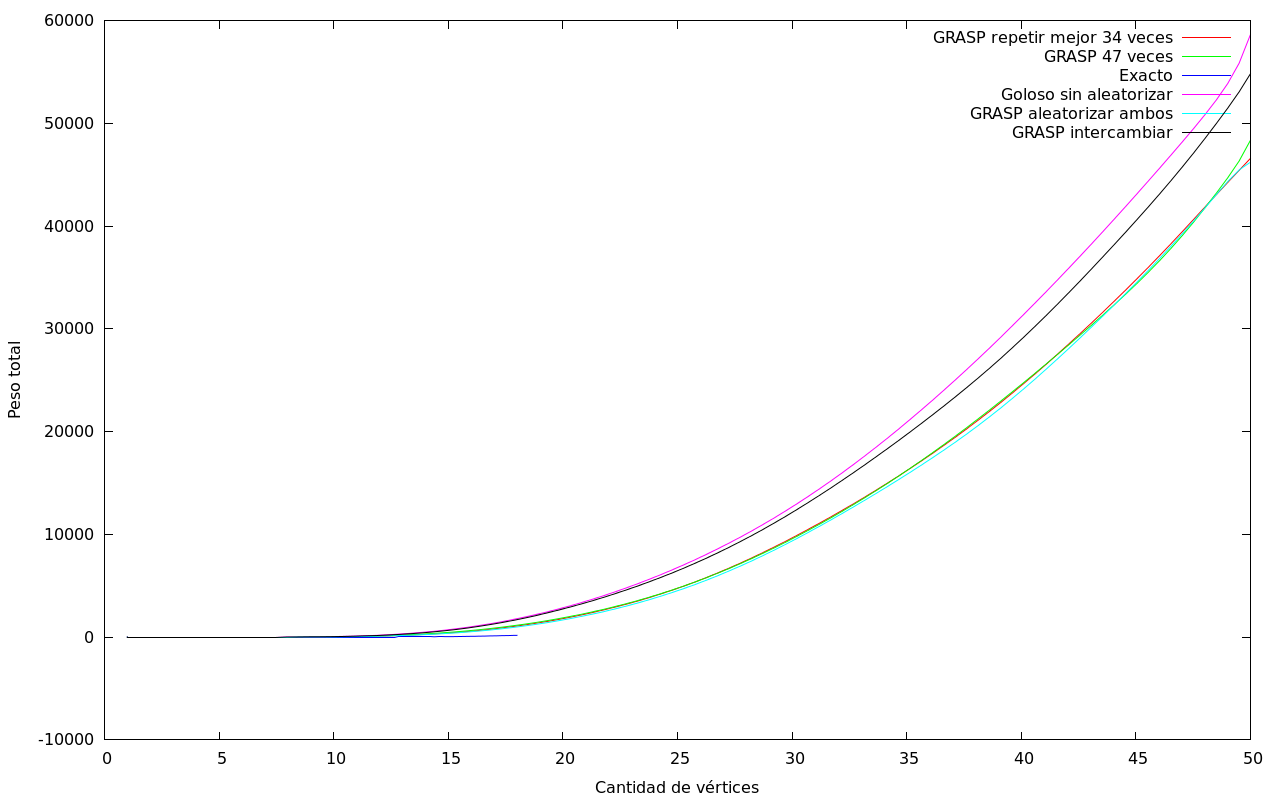
\includegraphics[scale=0.35]{imagenes/ej6-denso-pesos-distintos-k7-peso.png}
  \end{center}
\end{figure}

Lo primero que podemos notar es que en el árbol (un grafo bipartito, que puede
dividirse en 2 conjuntos y generar peso 0) y con $k = 3$, no todos llegan al
resultado obvio. Con $k = 7$ (no graficado) todos los algoritmos encuentran la
solución de peso 0.

Lo siguiente que se hace evidente es que ninguno logra llegar al resultado
exacto (para $n > 10$) y, sin embargo, dan resultados bastante similares,
ninguno crece en mayor medida que los otros.

Finalmente, el peor de todos, igualmente, es el goloso sin aleatorizar, seguido
del GRASP que utiliza la heurística de búsqueda local de \textit{intercambiar}.

Los otros tres algoritmos (los dos elegidos y GRASP, aleatorizando aristas y
conjuntos) tienen resultados muy parecidos, con diferencias menores al 1\% y
sin que ninguno tenga peso inferior consistentemente sobre los otros dos.

Considerando que la variación de GRASP que aleatoriza tanto aristas como
conjuntos era más lento que los otros dos, podemos confirmar que la elección
hecha fue la correcta: utilizando la meta-heurística GRASP, aleatorizando la
selección de aristas en el algoritmo goloso, usando la vecindad \textit{mover}
en el algoritmo de búsqueda local y sin importar el criterio de terminación,
pero dando un número considerable de repeticiones (34 y 47), obtuvimos los
mejores resultados en todas las pruebas.

Sin embargo, no fueron lo suficientemente buenas como para dar el resultado
exacto (o bastante cercano), por lo que queda abierto a mejoras.

Otro dato interesante es que la heurística golosa sin aleatorizar, aunque es
definitivamente la de peor calidad, la diferencia de peso total no es tan grande,
pero si lo es la diferencia en tiempos de ejecución, hasta 3 órdenes de magnitud
más rápido para grafos densos.
